\documentclass{standalone}
\usepackage{tikz}
\usetikzlibrary{patterns, positioning}
\usetikzlibrary{shapes.misc}
\usepackage[outline]{contour}
\contourlength{1.5pt} 


\begin{document}
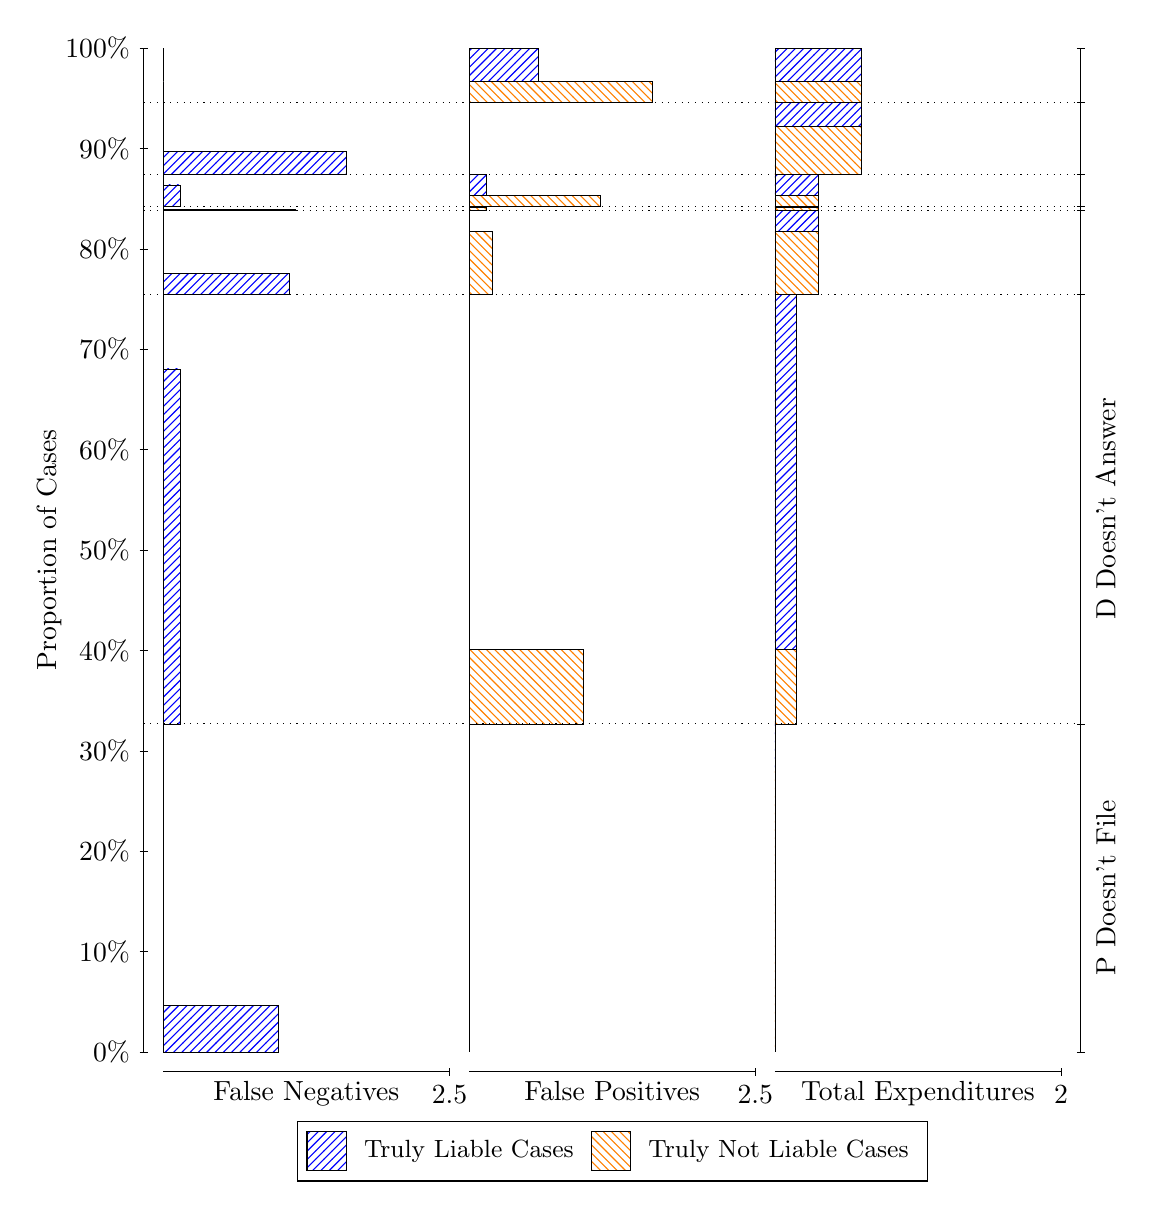
\begin{tikzpicture}
\draw[black, very thin] (1.5,1.75) -- (1.5,14.5);
\node[rotate=90, text=black, anchor=center] at (0.3, 8.125) {Proportion of Cases};
\draw[black, very thin] (1.45,1.75) -- (1.55,1.75);
\node[text=black, anchor=east] at (1.45, 1.75) {0\%};
\draw[black, very thin] (1.45,3.025) -- (1.55,3.025);
\node[text=black, anchor=east] at (1.45, 3.025) {10\%};
\draw[black, very thin] (1.45,4.3) -- (1.55,4.3);
\node[text=black, anchor=east] at (1.45, 4.3) {20\%};
\draw[black, very thin] (1.45,5.575) -- (1.55,5.575);
\node[text=black, anchor=east] at (1.45, 5.575) {30\%};
\draw[black, very thin] (1.45,6.85) -- (1.55,6.85);
\node[text=black, anchor=east] at (1.45, 6.85) {40\%};
\draw[black, very thin] (1.45,8.125) -- (1.55,8.125);
\node[text=black, anchor=east] at (1.45, 8.125) {50\%};
\draw[black, very thin] (1.45,9.4) -- (1.55,9.4);
\node[text=black, anchor=east] at (1.45, 9.4) {60\%};
\draw[black, very thin] (1.45,10.675) -- (1.55,10.675);
\node[text=black, anchor=east] at (1.45, 10.675) {70\%};
\draw[black, very thin] (1.45,11.95) -- (1.55,11.95);
\node[text=black, anchor=east] at (1.45, 11.95) {80\%};
\draw[black, very thin] (1.45,13.225) -- (1.55,13.225);
\node[text=black, anchor=east] at (1.45, 13.225) {90\%};
\draw[black, very thin] (1.45,14.5) -- (1.55,14.5);
\node[text=black, anchor=east] at (1.45, 14.5) {100\%};

\draw[black, very thin] (13.4,1.75) -- (13.4,14.5);
\draw[black, very thin] (13.35,1.75) -- (13.45,1.75);
\node[anchor=west] at (13.35, 1.75) {};
\draw[black, very thin] (13.35,5.9166) -- (13.45,5.9166);
\node[anchor=west] at (13.35, 5.9166) {};
\draw[black, very thin] (13.35,11.375) -- (13.45,11.375);
\node[anchor=west] at (13.35, 11.375) {};
\draw[black, very thin] (13.35,12.437) -- (13.45,12.437);
\node[anchor=west] at (13.35, 12.437) {};
\draw[black, very thin] (13.35,12.493) -- (13.45,12.493);
\node[anchor=west] at (13.35, 12.493) {};
\draw[black, very thin] (13.35,12.895) -- (13.45,12.895);
\node[anchor=west] at (13.35, 12.895) {};
\draw[black, very thin] (13.35,13.805) -- (13.45,13.805);
\node[anchor=west] at (13.35, 13.805) {};
\draw[black, very thin] (13.35,14.5) -- (13.45,14.5);
\node[anchor=west] at (13.35, 14.5) {};

\draw[black, very thin, pattern color=blue, pattern=north east lines] (1.75,1.75) rectangle (3.2033,2.3465);
\draw[black, very thin, pattern color=orange, pattern=north west lines] (1.75,2.3465) rectangle (1.75,5.9166);
\draw[black, very thin, pattern color=blue, pattern=north east lines] (1.75,5.9166) rectangle (1.968,10.425);
\draw[black, very thin, pattern color=orange, pattern=north west lines] (1.75,10.425) rectangle (1.75,11.375);
\draw[black, very thin, pattern color=blue, pattern=north east lines] (1.75,11.375) rectangle (3.3487,11.638);
\draw[black, very thin, pattern color=orange, pattern=north west lines] (1.75,11.638) rectangle (1.75,12.437);
\draw[black, very thin, pattern color=blue, pattern=north east lines] (1.75,12.437) rectangle (3.4213,12.455);
\draw[black, very thin, pattern color=orange, pattern=north west lines] (1.75,12.455) rectangle (1.75,12.493);
\draw[black, very thin, pattern color=blue, pattern=north east lines] (1.75,12.493) rectangle (1.968,12.762);
\draw[black, very thin, pattern color=orange, pattern=north west lines] (1.75,12.762) rectangle (1.75,12.895);
\draw[black, very thin, pattern color=blue, pattern=north east lines] (1.75,12.895) rectangle (4.0753,13.192);
\draw[black, very thin, pattern color=orange, pattern=north west lines] (1.75,13.192) rectangle (1.75,13.805);
\draw[black, very thin, pattern color=orange, pattern=north west lines] (1.75,13.805) rectangle (1.75,14.077);
\draw[black, very thin, pattern color=blue, pattern=north east lines] (1.75,14.077) rectangle (1.75,14.5);
\draw[black, very thin, pattern color=orange, pattern=north west lines] (5.6333,1.75) rectangle (5.6333,5.32);
\draw[black, very thin, pattern color=blue, pattern=north east lines] (5.6333,5.32) rectangle (5.6333,5.9166);
\draw[black, very thin, pattern color=orange, pattern=north west lines] (5.6333,5.9166) rectangle (7.0867,6.8668);
\draw[black, very thin, pattern color=blue, pattern=north east lines] (5.6333,6.8668) rectangle (5.6333,11.375);
\draw[black, very thin, pattern color=orange, pattern=north west lines] (5.6333,11.375) rectangle (5.924,12.173);
\draw[black, very thin, pattern color=blue, pattern=north east lines] (5.6333,12.173) rectangle (5.6333,12.437);
\draw[black, very thin, pattern color=orange, pattern=north west lines] (5.6333,12.437) rectangle (5.8513,12.475);
\draw[black, very thin, pattern color=blue, pattern=north east lines] (5.6333,12.475) rectangle (5.6333,12.493);
\draw[black, very thin, pattern color=orange, pattern=north west lines] (5.6333,12.493) rectangle (7.3047,12.625);
\draw[black, very thin, pattern color=blue, pattern=north east lines] (5.6333,12.625) rectangle (5.8513,12.895);
\draw[black, very thin, pattern color=orange, pattern=north west lines] (5.6333,12.895) rectangle (5.6333,13.508);
\draw[black, very thin, pattern color=blue, pattern=north east lines] (5.6333,13.508) rectangle (5.6333,13.805);
\draw[black, very thin, pattern color=orange, pattern=north west lines] (5.6333,13.805) rectangle (7.9587,14.077);
\draw[black, very thin, pattern color=blue, pattern=north east lines] (5.6333,14.077) rectangle (6.5053,14.5);
\draw[black, very thin, pattern color=orange, pattern=north west lines] (9.5167,1.75) rectangle (9.5167,5.32);
\draw[black, very thin, pattern color=blue, pattern=north east lines] (9.5167,5.32) rectangle (9.5167,5.9166);
\draw[black, very thin, pattern color=orange, pattern=north west lines] (9.5167,5.9166) rectangle (9.7892,6.8668);
\draw[black, very thin, pattern color=blue, pattern=north east lines] (9.5167,6.8668) rectangle (9.7892,11.375);
\draw[black, very thin, pattern color=orange, pattern=north west lines] (9.5167,11.375) rectangle (10.062,12.173);
\draw[black, very thin, pattern color=blue, pattern=north east lines] (9.5167,12.173) rectangle (10.062,12.437);
\draw[black, very thin, pattern color=orange, pattern=north west lines] (9.5167,12.437) rectangle (10.062,12.475);
\draw[black, very thin, pattern color=blue, pattern=north east lines] (9.5167,12.475) rectangle (10.062,12.493);
\draw[black, very thin, pattern color=orange, pattern=north west lines] (9.5167,12.493) rectangle (10.062,12.625);
\draw[black, very thin, pattern color=blue, pattern=north east lines] (9.5167,12.625) rectangle (10.062,12.895);
\draw[black, very thin, pattern color=orange, pattern=north west lines] (9.5167,12.895) rectangle (10.607,13.508);
\draw[black, very thin, pattern color=blue, pattern=north east lines] (9.5167,13.508) rectangle (10.607,13.805);
\draw[black, very thin, pattern color=orange, pattern=north west lines] (9.5167,13.805) rectangle (10.607,14.077);
\draw[black, very thin, pattern color=blue, pattern=north east lines] (9.5167,14.077) rectangle (10.607,14.5);
\draw[black, dotted] (1.5,5.9166) -- (13.4,5.9166);
\draw[black, dotted] (1.5,11.375) -- (13.4,11.375);
\draw[black, dotted] (1.5,12.437) -- (13.4,12.437);
\draw[black, dotted] (1.5,12.493) -- (13.4,12.493);
\draw[black, dotted] (1.5,12.895) -- (13.4,12.895);
\draw[black, dotted] (1.5,13.805) -- (13.4,13.805);
\draw[black, very thin] (1.75,1.5) -- (5.3833,1.5);
\node[text=black, anchor=north] at (3.5667, 1.5) {False Negatives};
\draw[black, very thin] (5.3833,1.45) -- (5.3833,1.55);
\node[text=black, anchor=north] at (5.3833, 1.45) {2.5};

\draw[black, very thin] (5.6333,1.5) -- (9.2667,1.5);
\node[text=black, anchor=north] at (7.45, 1.5) {False Positives};
\draw[black, very thin] (9.2667,1.45) -- (9.2667,1.55);
\node[text=black, anchor=north] at (9.2667, 1.45) {2.5};

\draw[black, very thin] (9.5167,1.5) -- (13.15,1.5);
\node[text=black, anchor=north] at (11.333, 1.5) {Total Expenditures};
\draw[black, very thin] (13.15,1.45) -- (13.15,1.55);
\node[text=black, anchor=north] at (13.15, 1.45) {2};

\node[text=black, centered, rotate=90] at (13.72, 3.8333) {\contour{white}{P Doesn't File}};
\node[text=black, centered, rotate=90] at (13.72, 8.6458) {\contour{white}{D Doesn't Answer}};






\draw (7.449999999999999,1.5) node[draw=none] (baseCoordinate) {};
\begin{scope}[align=center]
        \matrix[scale=0.5, draw=black, below=0.5cm of baseCoordinate, nodes={draw}, column sep=0.1cm]{
            \node[rectangle, draw, minimum width=0.5cm, minimum height=0.5cm, pattern color=blue, pattern=north east lines] {}; &
            \node[draw=none, font=\small, text=black] (B) {Truly Liable Cases}; &
            \node[rectangle, draw, minimum width=0.5cm, minimum height=0.5cm, pattern color=orange, pattern=north west lines] {}; &
            \node[draw=none, font=\small, text=black] (B) {Truly Not Liable Cases}; \\
            };
\end{scope}

\end{tikzpicture}
\end{document}